\documentclass[twocolumn]{jarticle}

\usepackage{proceeding}


\begin{document}

\pagestyle{empty}

\date{J--00}  %% 発表番号を記載しない場合は,{} 内を空欄とする.
\title{研究発表タイトル}
\author{高専 太郎,木更津 花子}
\maketitle

%% 現在ページの上部へのフロートの配置を抑制.
%% ここに記述しておくことで,最初のページの左段上部に図表を置かない.
\suppressfloats[t]


%%●●●●●●●●●●●●●●●
\section{まえがき}

文書領域の余白は,上 28 mm,下 24 mm,左右ともに 20 mm 空ける.

発表タイトルは 14 pt でセンタリングする.
%
フォントは,ゴシック体で,太字とする.
%
発表タイトルの下に 10 pt で 1 行分空ける.

発表者氏名は右端によせる.
%
発表者氏名の下に10 pt で1 行分空ける.

本文領域は 2 段組とし,段と段の間は 8 mm 空けることとする.

本文の章は「1. まえがき」から始めることとする.
%
また,本文の文章は 10 pt で記述することとし,行間は 1.5 mm とする.

ページ番号(フッタ)は用いないこと.
%
通し番号(「J--1」など)は後から印刷するので記述しなくてよい.


%%●●●●●●●●●●●●●●●
\section{研究概要}

章見出しは 12 pt,節見出しは 11 pt,項見出しは 10 pt を基本とする.
%
章番号とピリオドはいわゆる半角のCentury フォントを用いることとし,ピリオ
ドの後にいわゆる半角スペースを置いてから見出し語を書くこととする.
%
1.2 節がないのに,1.1 節を設けるのは論理的におかしいので注意すること.

英数字はいずれもいわゆる半角文字を用いること.

図のキャプションは図の下に表記すること(図~\ref{fig:test}).
%
逆に,表のキャプションは表の上に表記すること.
%
図,表のキャプションの説明文の最後にはいわゆる全角の句点を置く.
%
当然,図番号や表番号は本文中で引用しなければならない.

\begin{figure}[t]
 \begin{center}
  \includegraphics{test.eps}
  \caption{図のテスト.}
  \label{fig:test}
 \end{center}
\end{figure}

%%●●●●●●●●●●●●●●●
\section{まとめ}

参考文献の見出しには章番号は振らないことに注意する.
%
当然,参考文献で挙げた文献は,本文中で必ず引用すること.

参考文献は 9 pt とし,行間は 1 mm で列挙する.
%
文献名を囲む記号の開始は「``」であり,「''」ではない.
%
向きに注意して確認を怠らないようにする.

各項目の区切りは半角のカンマとスペースとし,最後は半角のピリオドとする.

複数の文献を同時に引用するとき,2 つまでは半角カンマで区切る
\cite{lit:一朗, lit:太郎}.
%
3 つ以上の場合は,ハイフンで最初と最後の文献番号を示す
\cite{lit:華子, lit:花子, lit:次郎, lit:三郎, lit:四郎}.


\begin{thebibliography}{9}
 \renewcommand{\baselinestretch}{1.0}
 \small
 \bibitem{lit:一朗}
	 情報 一朗,
	 ``「参考文献」の見出しには章番号をつけない'',
	 関東高専学会学会誌, Vol.5, pp.72--73, 2004.

 \bibitem{lit:太郎}
	 高専 太郎,
	 ``参考文献は 9 pt,行間 1 mm で記述する'',
	 日本高専学会学会誌, Vol.19, pp.88--91, 2005.

 \bibitem{lit:華子}
	 工学 華子,
	 ``囲む記号の開始記号の向きに注意'',
	 東日本高専学会学会誌, Vol.24, pp.54--55, 2003.

 \bibitem{lit:花子}
	 清見 花子,
	 ``区切りは半角のカンマとスペース'',
	 世界高専学会論文誌, Vol.34, pp.1006--1009, 2005.

 \bibitem{lit:次郎}
	 台東 次郎,
	 ``最後は半角ピリオド'',
	 宇宙高専学会技術報告, Vol.3, pp.12--15, 2006.

 \bibitem{lit:三郎}
	 木更 三郎,
	 ``URL での参考文献はなるべく避ける'', \\
	 \verb|http://www.kisarazu.ac.jp/|

 \bibitem{lit:四郎}
	 木更 四郎,
	 ``URL には下線を引かず,最後を示すピリオドも記述しない'', \\
	 \verb|http://www.j.kisarazu.ac.jp/|

\end{thebibliography}

\end{document}
